%!TEX root = thesis.tex
\chapter{Backgroud}
\section{\aclp{PAC}}
\aclp{PAC} are a relatively new class of controllers emerged in the past years
out of the discussion on advantages and disadvantages of \acp{PLC} compared to
\acp{PC} \citep{bel05}. The acronym \ac{PAC} itself was introduced by the
\ac{ARC} in 2001 \citep{pay13} to represent this next generation controllers.
However, a strict definition to clearly identify a \ac{PAC} and differentiate
it from other \acp{PLC} is missing. The term is used more as buzzword for the
automation vendor's marketing, but still reflects the increasing demands by
the modern industry and the evolution of automation controllers. 

Since its origin in the 1960s \citep{par99}, the \ac{PLC} dominates the
control and automation market by providing high reliability, a well-known
programming model and industrial I/O. It is used for various automation tasks
in typically electromechanical processes, for example machinery or plant
control. Inspired by the hand-wired relay logic systems and wire-diagrams, the
programming in ladder logic ease the transition to the new technology. Figure
\ref{fig:plc} shows the basic structure of a \ac{PLC} consisting out of input
and output ports and a program, implementing the control logic.
\begin{figure}
	\centering
	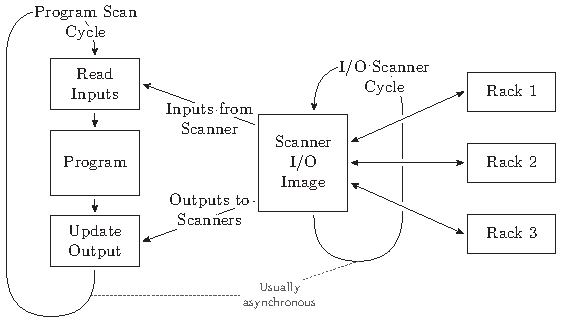
\includegraphics[width=5cm]{../figures/plc}
	\caption{The \acs{PLC} program scan \citep[adapted from][]{par99}}
	\label{fig:plc}
\end{figure}
The input ports are typically connected to different sensors, for example
light barriers, level indicators or temperature sensors, while the output
ports control actuators like contactors or valves. Each time the program scan
is executed, the inputs are read and fed into the control logic updating the
output ports accordingly. Note, that a \ac{PLC} does not control the system
continuously, but typically at a frequency of several $\SI{}{\kilo\hertz}$
\citep{par99}.

While the \ac{PLC} structure was designed for basic machine control, it
reaches its limits for more advanced applications requiring, for example,
extensive analog I/O, network connectivity, or enterprise integration. Back in
the 1980s and 1990s around 80\% of the industry's applications were solved by
traditional \acp{PLC} \citep{bel05}, resulting in a growth of low-cost systems
and a discontinuity in controller technology. Engineers targeting the 20\% of
feature rich applications pushed the classical designs to its limits.
Consequently, they started evaluating different technology and came up with
\acp{PC} for industrial control, offering advanced software capabilities,
utilization of \ac{COTS} components and graphical environments \citep{bel05}.
However, standard \acp{PC} are not ideal for industrial control applications
due to missing robustness in rugged environments, stable operating systems and
common programming environments. Finally, the engineers either omitted
advanced functionalities or deployed a coupled \ac{PC}/\ac{PLC} system.
Without any satisfactory solution, the engineers worked together with hardware
vendors to develop

\begin{figure}
	\centering
	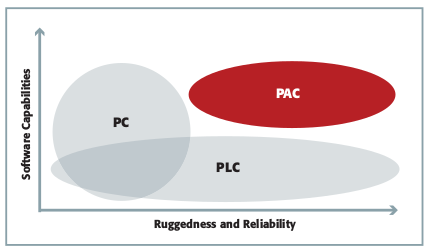
\includegraphics[width=5cm]{../figures/pac}
	\caption{\acp{PAC} compared to \acp{PLC} and \acp{PC} \citep[adapted from][]{bel05}}
	\label{fig:pac}
\end{figure}
\begin{itemize}
\item In 1969 developed based on a specification for an industrial computer  produced by General Motors \citep{par99}\\
\lstinline{http://books.google.de/books?id=zLwtngK3T1UC&printsec=frontcover&hl=de&source=gbs_ge_summary_r&cad=0#v=onepage&q=programmable%20logic&f=false}
\item \acp{PLC} dominate market of automation and control
\item brief explanation what PLC is doing (input, loop, ouput, ...)
\item Growing demands show limits of \acp{PLC} (Web-based, database, ...)
\item For 20 percent of advanced applications (rest only small, low cost)

\item PCs arrive, not suitable (OS not stable, rugged environment, complexity)
\item $\Rightarrow$ live without functionality or combine PC and PLC
\item \acp{PAC} as combination of PLC and PC
\item Custom hardware goes away (incorporation of FPGAs)
\item $\Rightarrow$ emphasize this with paper hybrid2.pdf
\item Complex system, hardware software boundary
\item abstraction of hardware and software
\item multithreaded programming model
\item ReconOS as framework for hybrid multi-core systems
\end{itemize}

\section{ReconOS}
\begin{itemize}
\item Multithreaded Programming model
\item Abstraction form hardware software boundary
\item ...
\end{itemize}

\section{High Level Synthesis}